\documentclass[10pt]{article}
\usepackage[margin=1in]{geometry} 

\usepackage{amsmath,amsthm,amssymb,graphicx,amsfonts}

\usepackage{float}
\usepackage{caption,subcaption} % para las figuras
\usepackage{wrapfig}

\usepackage{comment}

\usepackage[utf8]{inputenc} %tildes
\usepackage[spanish]{babel}

\usepackage{enumerate}

\usepackage{color}   %May be necessary if you want to color links
\usepackage[hyphens]{url}
\usepackage[hidelinks]{hyperref}
\hypersetup{breaklinks=true}
\urlstyle{same}

\hypersetup{
	colorlinks=true, %set true if you want colored links
	linktoc=all,     %set to all if you want both sections and subsections linked
	linkcolor=blue,  %choose some color if you want links to stand out
}

\begin{document}
	
\title{Población Penitenciaria en Argentina\\ 2002 a 2017 \\
	\begin{small}
		Tutor: Franco Camporeale
	\end{small}}
\author{\small{Nahuel Almeira, María Lucía Pappaterra, Javier Y\'anover}}

\maketitle

\section{Análisis estadístico de variables}

Seleccionar un conjunto de al menos cuatro variables que resulten de interés.

\begin{enumerate}
	\item Usar distintos tipos de gráficos para describir sus distribuciones
	\item Analizar Outliers
	\item Calcular estadísticos clásicos (media, mediana, moda, desviación estandar)
\end{enumerate}

Las variables elegidas fueron: edad, duración de condena, diferencia entre fecha de condena y fecha de detención, cantidad de delitos por interno.

\subsection{Edad}

En la figura \ref{fig:edad} mostramos la distribuci\'on de edades de los internos, junto con su suma acumulada. Podemos ver que la mayor\'ia de los internos son personas j\'ovenes, y que el n\'umero de internos decae fuertemente con la edad. En el histograma se observa que hay registros de personas con edad cercana a 0 años. En realidad, se trata de 369 registros con edad igual a 0 años. Estos casos podr\'ian tratarse de un error de carga, o podr\'ian corresponder a ni\~nos nacidos dentro de los establecimientos. Observando en detalle esos registros, se puede ver que la segunda opci\'on es improbable, dado que esos registros tienen informaci\'on en otros campos que corresponden a internos que han cometido delitos.  Los dem\'as registros que podr\'ian ser considerados como outliers son los correspondientes a menores de edad. En este caso, existen 8 registros de personas de 16 a\~nos y 11 registros de personas de 17 a\~nos. Como esta cantidad es baja y no afecta la estad\'istica, decidimos incluirlos en el an\'alisis.

\begin{figure}[H]
	\centering
	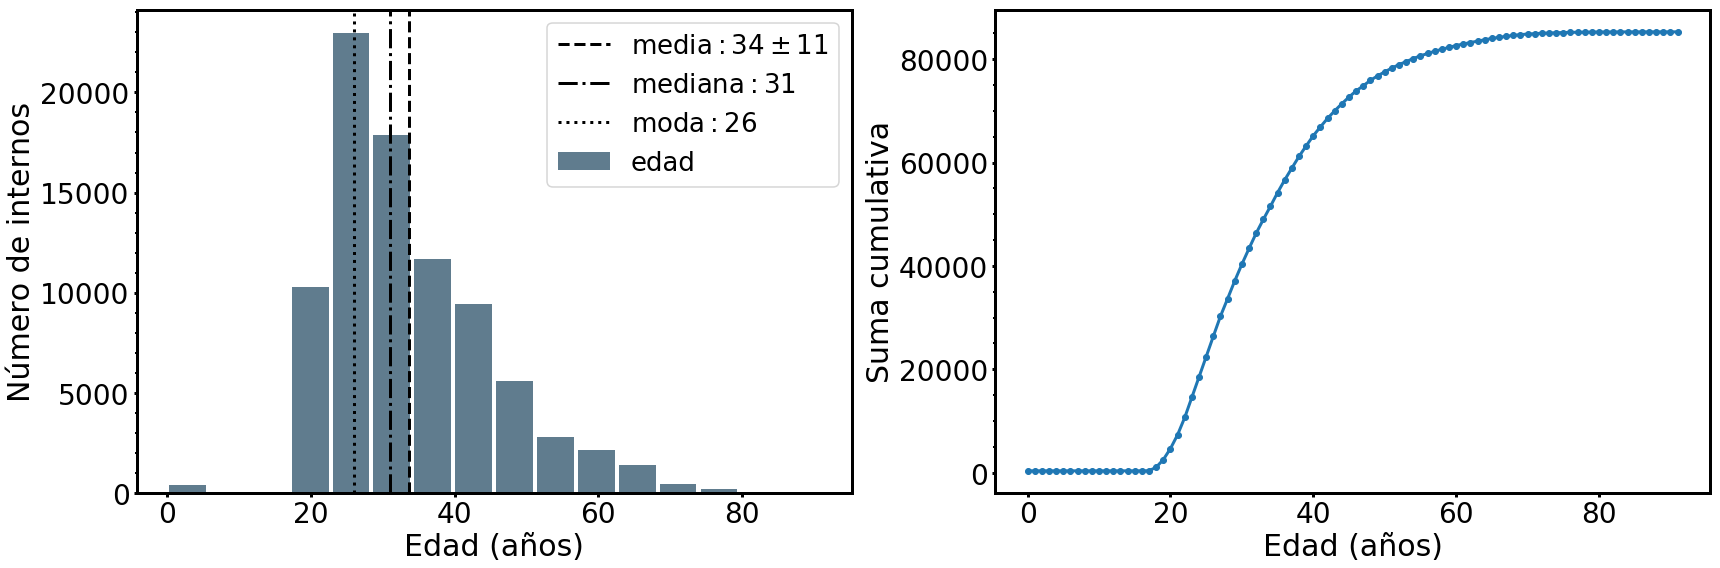
\includegraphics[scale=0.26]{graficos/edad.png}
	\caption{Histograma de edades de los internos, junto con su la suma acumulada. \label{fig:edad}}
\end{figure}

\subsection{Duración de condena}

Para estudiar la duraci\'on de las condenas, es necesario utilizar dos campos: ``duracion\textunderscore condena\textunderscore anios'', que indica la cantidad de a\~nos completos, y ``duracion\textunderscore  condena\textunderscore  meses'', que indica la cantidad de meses restantes. Por ejemplo, una condena de 9 a\~nos y 5 meses figurar\'ia en la base de datos como duracion\textunderscore  condena\textunderscore  anios: 9, duracion\textunderscore  condena\textunderscore  meses: 5. Para nuestro an\'alisis, consideramos una nueva variable racional que sea la suma de los dos campos anteriores, medida en a\~nos. 

El preprocesamiento fue el siguiente: Filtramos los registros con valor nulo en duracion\textunderscore condena\textunderscore anios (1) y con valor nulo en duracion\textunderscore condena\textunderscore meses (32). Luego, filtramos los registros con valor igual a 0 en ambos campos (3649).

En la figura \ref{fig:duracion_condena} mostramos el histograma de duraci\'on de condenas, junto con su suma cumulativa complementaria. Podemos ver que la mayor\'ia de las condenas son cortas (las tres medidas de centralidad calculadas son menores o iguales a 8 a\~nos), y que presentan un decaimiento aproximadamente exponencial a medida que se incrementa la duraci\'on. 

\begin{figure}[H]
	\centering
	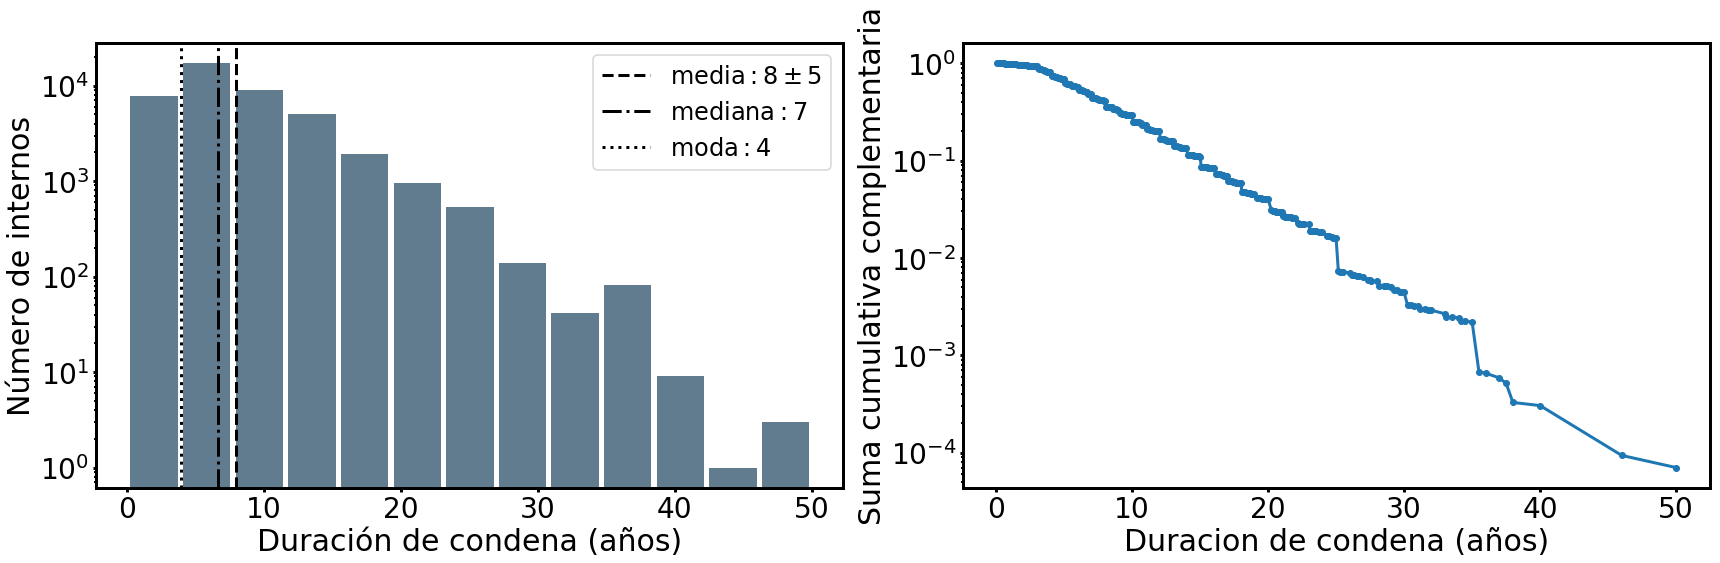
\includegraphics[scale=0.26]{graficos/duracion_condena.png}
	\caption{Histograma de la duraci\'on de condenas y su suma cumulativa complementaria. \label{fig:duracion_condena}}
\end{figure}

\subsection{Diferencia entre fecha de condena y fecha de detenci\'on}

Una importante fracci\'on de la poblaci\'on penal se encuentra detenida sin una condena firme. La situaci\'on m\'as frecuente es la de la prisi\'on preventiva. A continuaci\'on, mostramos un an\'alisis sobre los tiempos transcurridos entre la detenci\'on y la aplicaci\'on de la condena. Para ello, utilizamos los campos ``fecha\textunderscore detencion'' y ``fecha\textunderscore condenado''.

Preprocesamiento: Seleccionamos s\'olo los registros cuya situaci\'on penal sea ``Condenado'' (46405). Luego filtramos aquellos que tengan valores nulos para cualquiera de los dos campos de inter\'es. En tercer lugar, filtramos los registros que tengan fechas posteriores a la fecha del censo (6409). Estos \'ultimos casos son claramente outliers y corresponde descartarlos.

Al observar la distribuci\'on de diferencias de tiempo (figura \ref{fig:tiempo_detencion_condena}) se puede ver que hay una gran cantidad de casos con diferencia de tiempo negativas. De hecho, la distribuci\'on est\'a centrada en un valor cercano a cero, y decae aproximadamente tanto hacia valores positivos como negativos. Mientras que los valores positivos no parecen, a priori, extraños, es necesario interpretar los valores negativos. Para esto, hay que preguntarse si existe alguna condición en la que la fecha de condenado pueda preceder a la fecha de detención. 

\begin{figure}[H]
	\centering
	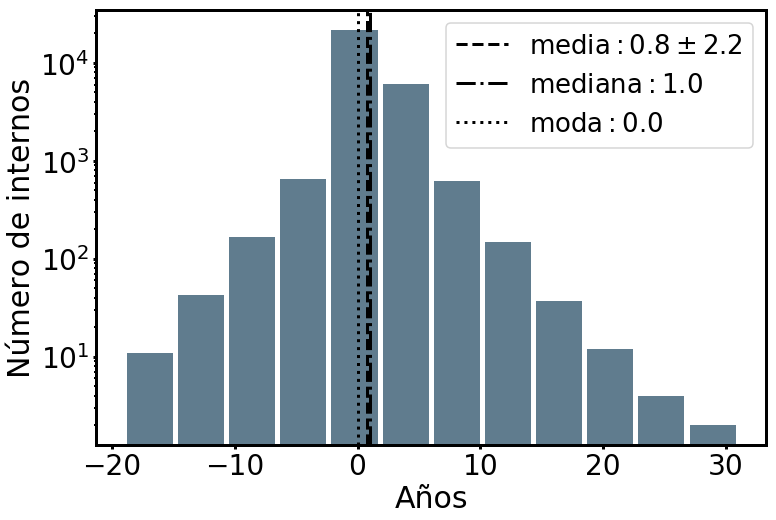
\includegraphics[scale=0.3]{graficos/diff_condenado_detencion_negativos.png}%
	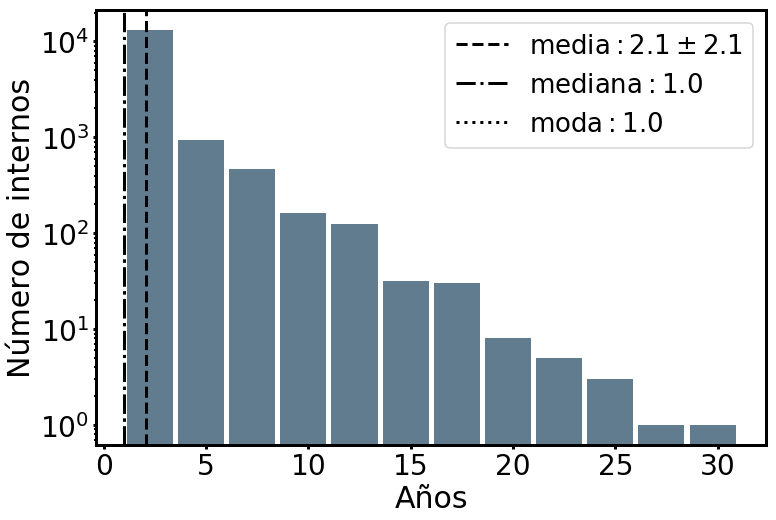
\includegraphics[scale=0.3]{graficos/diff_condenado_detencion.png}
	\caption{Histograma de los tiempos transcurridos entre la fecha de detenci\'on y la fecha de condena. A la izquierda, teniendo en cuenta diferencias de tiempo negativas, y a la derecha, considerando s\'olo las positivas. \label{fig:tiempo_detencion_condena}}
\end{figure}


Existen algunas hipótesis que podrían dar lugar a una situación de este tipo. La primera es que una persona podría haber recibido la condena sin estar detenida, o estando detenida en un establecimiento policial, cuyos datos no están dentro de la base de datos, y haber sido incorporada al servicio penitenciario un tiempo después. Podría suceder, incluso, que una persona se de a la fuga después de haber sido condenada, y antes de ser detenida. La segunda es que una persona puede tener múltiples causas. Se puede dar el caso en que una persona haya sido condenada por una causa y que, habiendo cumplido su condena, haya sido detenida por un segundo delito. En ese caso, podría ser que el registro muestre la fecha de condena de la primera causa, y la fecha de detención de la segunda. Para testear esta hipótesis, se podría estudiar si los registros para los cuales la diferencia de tiempos es negativa corresponde a registros de reincidentes. La tercera es que un condenado haya sido derivado de otro establecimiento y que figure como fecha de detención la fecha en la que ingresó al último establecimiento.

Para este primer análisis, vamos a considerar todos los valores negativos como outliers y descartarlos. Más adelante, buscaremos evaluar estas hipótesis. Al hacer esto, obtenemos la gr\'afica de la derecha en la figura \ref{fig:tiempo_detencion_condena}.


\subsection{Cantidad de delitos por interno}

Cada interno puede haber cometido uno o más delitos. Cada delito está registrado en un campo distinto, y se registra hasta un máximo de 5 delitos, ordenados de mayor a menor gravedad\footnote{No en todos los casos la clasificaci\'on est\'a bien hecha. De hecho, existen regsitros donde el primer delito es nulo, y el segundo no lo es.}. Aquí veremos cómo se distribuye el número de delitos por interno.

En el histograma de la figura \ref{fig:cantidad_delitos} podemos ver el histograma con la cantidad de delitos por interno. Vemos que la gran mayor\'ia (68915 registros) ha cometido un \'unico delito, y que este n\'umero decae de manera aproximadamente exponencial para delitos mayores que 1.  

\begin{figure}[H]
	\centering
	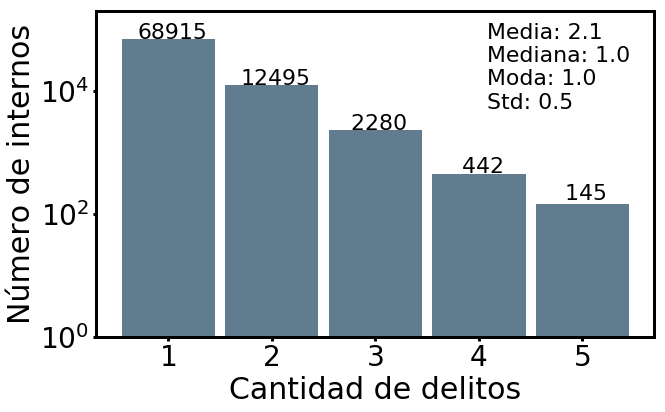
\includegraphics[scale=0.4]{graficos/cantidad_delitos.png}
	\caption{Histograma de la cantidad de delitos cometidos por cada interno. \label{fig:cantidad_delitos}}
\end{figure}

\section{Evolución de variables en el tiempo}

Seleccionar dos variables y graficar cómo fueron cambiando desde 2002 a 2017. Para ello se tiene que utilizar el siguiente conjunto de datos: \url{https://github.com/camporeale/Datos/raw/master/sneep_2002_2017_diplodatos.zip}\\

Las variables elegidas fueron la situación legal y la participación en programas educativos.

\subsection{Situación legal}

Como mencionamos anteriormente, un gran n\'umero de internos se encuentra detenido sin condena firme. Esta situaci\'on no es nueva, sino que existe desde hace por los menos 15 a\~nos (desde que se comenz\'o a realizar el censo). De hecho, de acuerdo con una nota de la plataforma Chequeado \cite{chequeadoCondenados}, esta situaci\'on era m\'as significativa en el pasado, y se ha ido revirtiendo con los a\~nos. Como podemos apreciar de la figura \ref{fig:situacion_legal}, nuestro an\'alisis coincide con el de la nota period\'istica. En particular, podemos observar que hist\'oricamente, m\'as de la mitad de los internos estuvo detenido sin condena. Esta situaci\'on se revierte reci\'en en el a\~no 2016.

\begin{figure}[H]
	\centering
	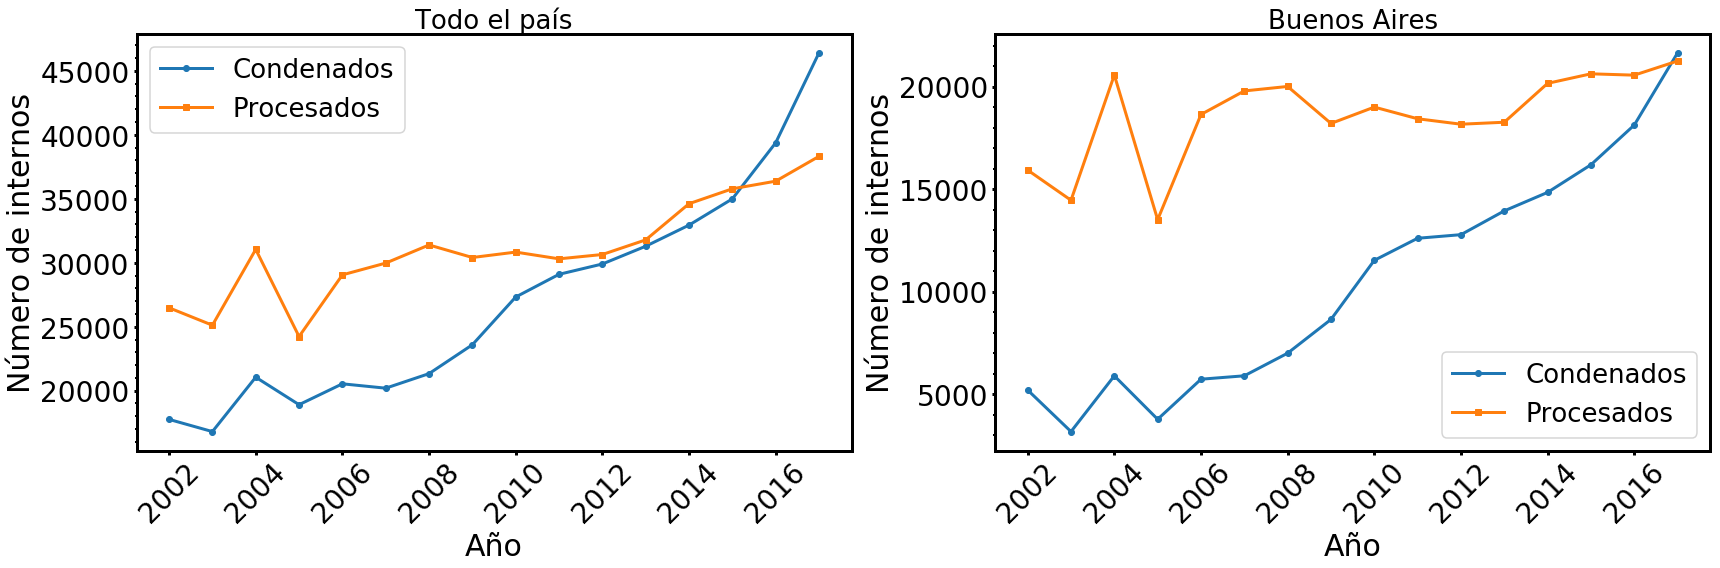
\includegraphics[scale=0.26]{graficos/situacion_legal.png}
	\caption{Cantidad de internos en funci\'on del tiempo, discriminados por su situaci\'on legal. \label{fig:situacion_legal}}
\end{figure}


\subsection{Participación en programas educativos}

Queremos ver cómo varía la proporción de internos que participa en programas educativos a lo largo del tiempo. Los programas se clasifican de acuerdo a educaci\'on formal (primaria, secundaria, terciaria y universitaria) y no formal.

En la figura \ref{fig:educativos} podemos ver la evoluci\'on temporal de la participaci\'on en cada uno de los programas. Mientras que los programas de educaci\'on no formal no presentan una variaci\'on significativa en el tiempo. los programas de educaci\'on formal presentan un incremento. Al desglosar los distintos tipos de educaci\'on formal, vemos que el incremento m\'as significativo se da en el nivel medio. Por otro lado, también se observa que la proporción de internos involucrados en estudios primarios y secundarios es mucho mayor que la de terciarios y universitarios.

\begin{figure}[H]
	\centering
	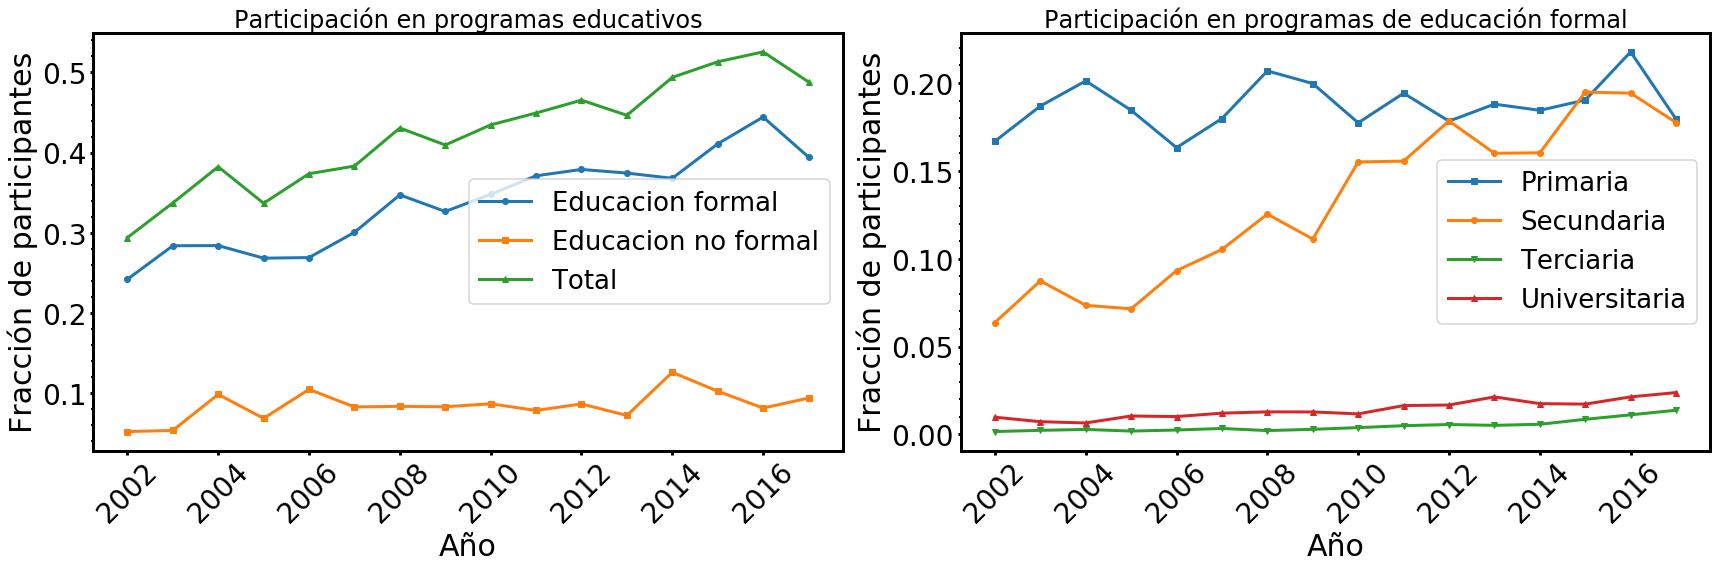
\includegraphics[scale=0.26]{graficos/participacion_educativos.png}
	\caption{Participaci\'on en diferentes programas educativos dentro de los establecimientos penitenciarios.\label{fig:educativos}}
\end{figure}

\section{Análisis de probabilidades condicionales}

Tomar al menos dos pares de variables y realizar un análisis del tipo:

\begin{itemize}
	\item ¿Cuál es la probabilidad de que el interno haya sido lesionado en el último año dado que está en una prisión en Buenos Aires? ¿Y en Córdoba?
	\item ¿Cuál es la probabilidad de que se le otorguen salidas provisorias dado que esté casado/a? ¿Y siendo soltero?
\end{itemize}

El primer par de variables que elegimos es el par nacionalidad vs. tipo de establecimiento (federal o no federal). En concreto, queremos ver c\'omo cambia la poblaci\'on penal, en relaci\'on a la nacionalidad de los internos, seg\'un el tipo de establecimiento que se trate. 

En el gr\'afico de barras de la figura \ref{fig:nacionalidad_todos}, mostramos los porcentajes de internos de acuerdo a su nacionalidad. Podemos ver que la gran mayor\'ia (m\'as del 94\%) son de nacionalidad argentina. Del porcentaje restante, la mayor parte se distribuye entre paraguayos, peruanos y bolivianos. Para una mejor visualizaci\'on, descartamos las nacionalidades con poblaci\'on menor al $0.01\%$.

\begin{figure}[H]
	\centering
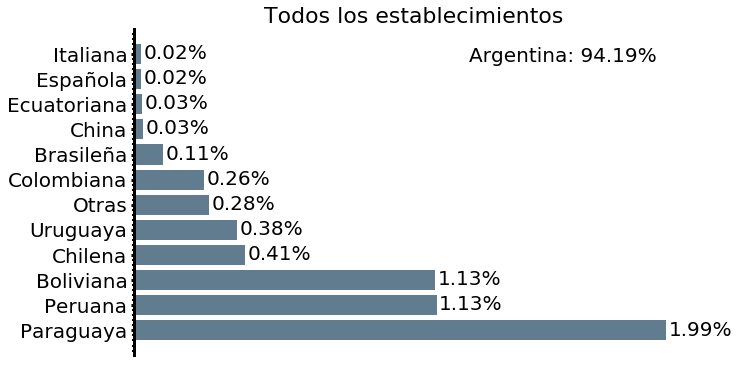
\includegraphics[scale=0.40]{graficos/nacionalidad_bar.png}
	\caption{Porcentaje de internos de acuerdo a su nacionalidad, considerando todos los establecimientos penales.\label{fig:nacionalidad_todos}}
\end{figure}

En el a\~no 2014, el senador Miguel \'Angel Pichetto mencion\'o en una entrevista que el 20\% de la poblaci\'on penal eran inmigrantes. Basado en ese dato, sostuvo la necesidad de fortalecer el control fronterizo para disminuir el delito (particularmente, el narcotr\'afico) en Argentina. El dato mencionado es incorrecto, tal como se menciona en la nota de Chequeado \cite{chequeadoInmigrantes}. Si bien los datos que ac\'a presentamos no corresponden al mismo per\'iodo, se puede hacer un an\'alisis similar al de la nota. B\'asicamente, el dato presentado por Pichetto en realidad corresponde a la poblaci\'on penal perteneciente a establecimientos federales, donde la proporci\'on de inmigrantes es mayor, tal como se puede ver en la figura \ref{nacionalidad_discriminado}. 

\begin{figure}[H]
	\centering
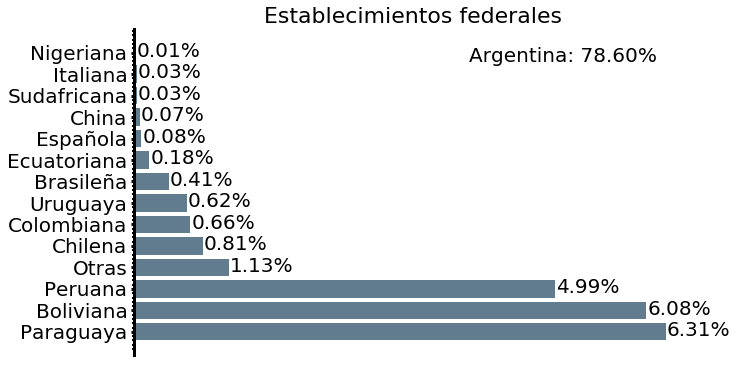
\includegraphics[scale=0.31]{graficos/nacionalidad_bar_federales.png}
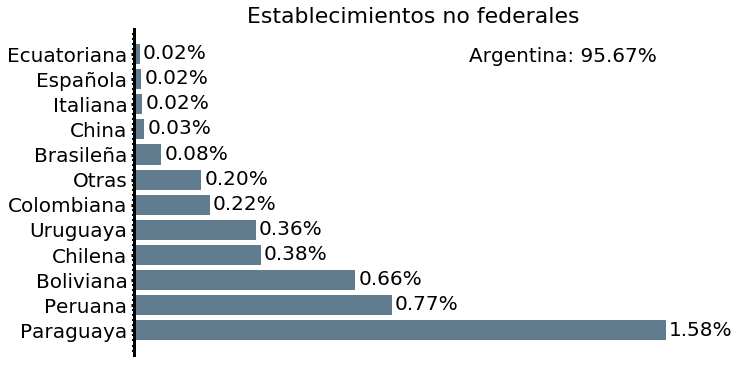
\includegraphics[scale=0.31]{graficos/nacionalidad_bar_no_federales.png}
	\caption{Porcentaje de internos de acuerdo a su nacionalidad, discriminando establecimientos federales de no federales.\label{nacionalidad_discriminado}}
\end{figure}

Continuando con el an\'alisis, analizamos si en verdad los inmigrantes cometen en mayor medida delitos asociados a la ley de estupefacientes $\mathrm{N}^{\circ}\; 23737$. En la figura \ref{estupefacientes_discriminado} podemos observar que la poblaci\'on carcelaria extranjera s\'i ha cometido, en mayor proporci\'on delitos asociados a esta ley. Sin embargo, la informaci\'on disponible no permite diferenciar los delitos de ``microtr\'afico'', o peque\~na venta de drogas, de lo que se conoce como ``narcotr\'afico'', dado que ambas categor\'ias caen dentro de la misma ley. 

\begin{figure}[H]
	\centering
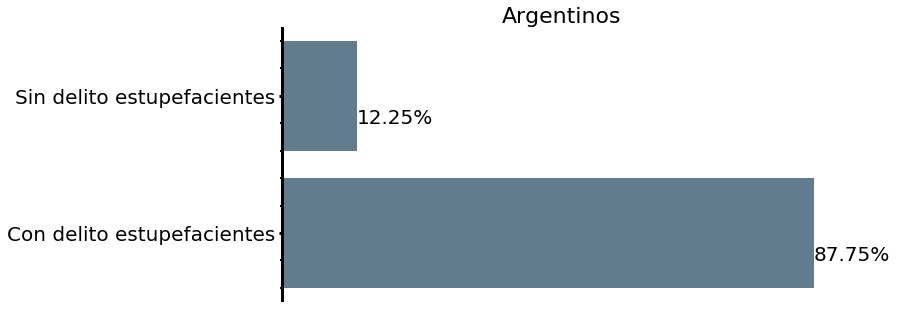
\includegraphics[scale=0.28]{graficos/estupefacientes_bar_argentinos.png}
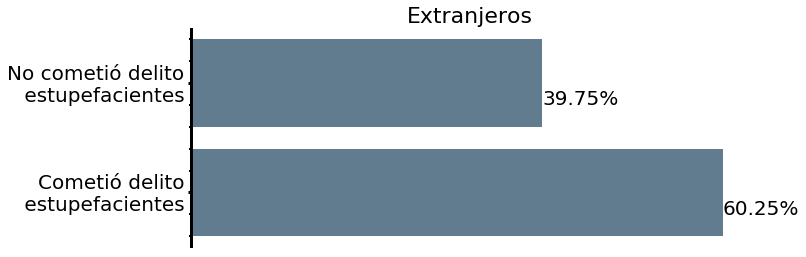
\includegraphics[scale=0.28]{graficos/estupefacientes_bar_extranjeros.png}
	\caption{Porcentaje de internos detenidos o condenados por delitos asociados a la ley de estupefacientes $\mathrm{N}^{\circ}\; 23737$, discriminado seg\'un nacionalidad.\label{estupefacientes_discriminado}}
\end{figure}

\Urlmuskip=0mu plus 1mu\relax
\bibliography{referencias}
\bibliographystyle{ieeetr}


\end{document}